\documentclass[12pt,a4paper]{article}
\usepackage[ngerman]{babel}
\usepackage[utf8]{inputenc}
\usepackage[unicode=true,bookmarks=false,bookmarksopen=true]{hyperref}

\usepackage{xcolor}
\usepackage{graphicx}
\usepackage{tikz}

\usepackage{listings}

\def\checkmark{\tikz\fill[scale=0.4](0,.35) -- (.25,0) -- (1,.7) -- (.25,.15) -- cycle;}

\definecolor{pGreen}{rgb}{0.44, 0.71, 0}
\definecolor{nRed}{rgb}{0.74, 0, 0}

\title{ORES Custom Documentation VI}
%\author{Tom Gülenman}
\date{}
\begin{document}
\maketitle
\textit{Disclaimer: No guarantee for the correctness of information / explanations / sources is given.}\\
%
\section*{Goals}
\begin{enumerate}
\item Metrics List: Create Table as a general quickview \checkmark
\item Metrics: which combinations are particularly useful, which are nonsensical?
\begin{itemize}
\item Ask for documentation on IRC (\checkmark)
\item Logically exclude combinations?
\item Document outputs
\end{itemize}
\item Recent Changes filter classes: how are edits assigned to them?
\begin{itemize}
\item Also ask for documentation on IRC \checkmark
\item Which metrics are included in the process? \checkmark
\item How are the metrics (precision, recall, threshold) included in the associated API calls? What do the (GET?)-Requests look like?
\end{itemize}
\item Take a closer look at the Threshold Plot for Logistic Regression (\href{http://www.scikit-yb.org/en/latest/api/classifier/threshold.html}{Link})
\begin{itemize}
\item What is the meaning of the areas around the curves? \checkmark
\item What is queue rate exactly? \checkmark
\end{itemize}
\item Take a closer look at the Swagger API Documentation
\item \colorbox{red}{ !!! } Improve knowledge of ORES Docs and foremost the metrics
\end{enumerate}
%
%
%
\newpage
\section{Metrics List: Table}
\begin{tabular}{|l|l|c|}
\hline
\textbf{Metric} & \textbf{Quick Definition} & \textbf{Value}\\\hline \hline
accuracy & Portion of correctly predicted data & $\frac{\texttt{TP}+\texttt{TN}}{\texttt{Total}}$\\\hline
counts & Number of \textbf{F}\&\textbf{T}-labels and predictions&\\\hline
f1 & Harmonic mean of recall and precision & $2*\frac{\texttt{rec} * \texttt{prec}}{\texttt{rec}+\texttt{prec}}$\\\hline
filter\_rate & Portion of observations predicted & $1-\texttt{match\_rate} =$\\ &to be negative&$\frac{\texttt{TN}+\texttt{FN}}{\texttt{Total}}$\\\hline
fpr & Probability of a false alarm & $\frac{\texttt{FP}}{\texttt{FP} + \texttt{TN}}$\\\hline
match\_rate & Portion of observations predicted & $\frac{\texttt{TP}+\texttt{FP}}{\texttt{Total}}$\\ &to be positive&\\\hline
pr\_auc & Measure of classification performance &\\\hline
precision & Ability to find only relevant cases & $\frac{\texttt{TP}}{\texttt{TP} + \texttt{FP}}$\\\hline
rates & Proportion of \textbf{F}\&\textbf{T}-labels to the total&\\\hline
recall & Ability to find \textbf{all} relevant cases & $\frac{\texttt{TP}}{\texttt{TP} + \texttt{FN}}$\\\hline
roc\_auc & Measure of classification performance &\\\hline
!f1 & Negated f1 & $2*\frac{\texttt{!rec} * \texttt{!prec}}{\texttt{!rec}+\texttt{!prec}}$\\\hline
!precision & Negated precision & $\frac{\texttt{TN}}{\texttt{TN} + \texttt{FN}}$ \\\hline
!recall & Negated recall & $\frac{\texttt{TN}}{\texttt{TN} + \texttt{FP}}$\\\hline
\end{tabular}
%
%
%
\section{Metrics combinations}
example: \url{https://ores.wikimedia.org/v3/scores/enwiki/?models=damaging&model_info=statistics.thresholds.true.%27maximum%20!precision%20@%20precision%20%3E=%200.9%27}
%TODO
%TODO also see https://www.mediawiki.org/wiki/ORES/Thresholds -> worked example
More links for quickstart:
\begin{itemize}
\item \href{https://ores.wikimedia.org/v3/scores/enwiki/?models=damaging&model_info=statistics.thresholds.true}{1}
\item \href{https://upload.wikimedia.org/wikipedia/commons/2/26/Precisionrecall.svg}{2}
\item \href{https://ores.wikimedia.org/v3/scores/enwiki/?models=damaging&model_info=statistics.thresholds.true.%27maximum%20!precision%20@%20precision%20%3E=%200.9%27}{3}
\item \href{https://ores.wikimedia.org/v3/scores/enwiki/?models=damaging&model_info=statistics.thresholds.true.%27maximum%20filter_rate%20@%20recall%20%3E=%200.75%27}{4}
\end{itemize}
%
%
%
\section{Recent Changes Quality Prediction Filters}
The Recent Changes quality prediction filters are a helpful tool in varying the precision and recall of catching damaging edits. They can be applied on the Recent changes site (\href{https://en.wikipedia.org/wiki/Special:RecentChanges?hidebots=1&hidecategorization=1&hideWikibase=1&limit=50&days=7&urlversion=2}{Link}).\\
\\
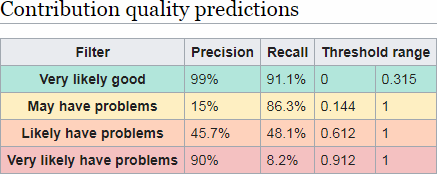
\includegraphics[scale=0.85]{resources/6/RCFilters}\\
{\href{https://en.wikipedia.org/wiki/Special:ORESModels}{Wikipedia Source}
\subsection{Precision and Recall}
To put those numbers into context: we can expect that, for example, the \textit{Likely have problems} filter will be right about $45.7\%$ of the time, classifying a contribution as damaging while catching $48.1\%$ of problem edits.\\

\subsection{Threshold ranges}
Keep in mind that the damaging model classifier is binary, deciding wether a contribution is damaging or not, but does not only output 0 or 1, but instead a probability (between 0 and 1) of how probable it is, that a contribution is damaging. The threshold then decides at which probability the contributions are split into damaging and non-damaging (e.g. a threshold of 0.6 means that every contribution with a value of under 0.6 will be classified as non-damaging and vice versa). Threshold ranges therefore signify the following: 
\begin{itemize}
\item \textit{Very likely good}: Contributions that score between 0 and 0.315 on the probability-of-being-damaging scale
\item \textit{May have problems}: Contributions that score between 0.144 and 1
\item \textit{Likely have problems}: Contributions that score between 0.612 and 1
\item \textit{Very likely have problems}: Contributions that score between 0.912 and 1
\end{itemize}

To better understand threshold ranges it's helpful to also take a look at the following graphic:\\
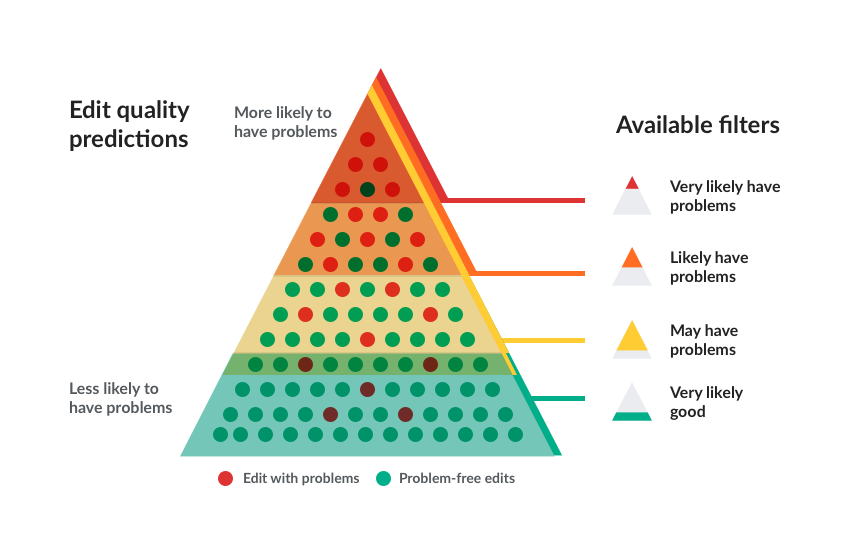
\includegraphics[scale=0.5]{resources/6/RC-quality-filters-diagram}\\
\href{https://upload.wikimedia.org/wikipedia/commons/e/e8/RC-quality-filters-diagram.png}{Wikimedia Source}, \href{https://www.mediawiki.org/wiki/Help:New_filters_for_edit_review/Quality_and_Intent_Filters}{MediaWiki Source}\\
Note two things:
\begin{enumerate}
\item The \textit{May have problems}, \textit{Likely have problems}, and \textit{Very likely have problems} filters overlap.
\begin{description}
\item More precisely, the most general filter \textit{May have problems} contains all edits that also are part of the other two filters and, similarly, edits of \textit{Very likely have problems} are a subset of \textit{Likely have problems}.
\end{description}
\item The \textit{Very likely good} and \textit{May have problems} filters overlap.
\begin{description}
\item This overlap is referred to as ``the indeterminate zone between problem and problem-free edits'' and happens in order to achieve a ``broader recall''.
\end{description}
\end{enumerate}
\subsection{Highlighting}
It is also possible to apply filters, for example the broadest one \textit{May have problems} and then highlight edits marked as particularly alarming by using color highlighting for the \textit{Likely have problems} and \textit{Very likely have problems} filters.\\
Read more on highlighting: \href{https://www.mediawiki.org/wiki/Help:New_filters_for_edit_review/Highlighting_function}{Mediawiki Link}.
\subsection{Recent Changes ORES Requests}
Here is how it is decided to which filter category contributions belong:
\begin{enumerate}
\item MediaWiki sends requests to ORES, as soon as edits are saved, to get the \textbf{score.probability.true} of edits. (See source: \href{https://github.com/wikimedia/mediawiki-extensions-ORES/blob/master/includes/FetchScoreJob.php}{MediaWiki Request to ORES})
\item The value of \textbf{score.probability.true} is then stored in a table (ores\_classification table) that can be joined to the recent\_changes table.
\item Having the threshold ranges for all available filters, an edit's \textbf{score.probability.true} has to be a value in the threshold ranges interval for the edit to be a part of that filter category.
\end{enumerate}
%
%
%
\section{\href{http://www.scikit-yb.org/en/latest/api/classifier/threshold.html}{Discrimination Threshold Visualisation (Logistic Regression)}}
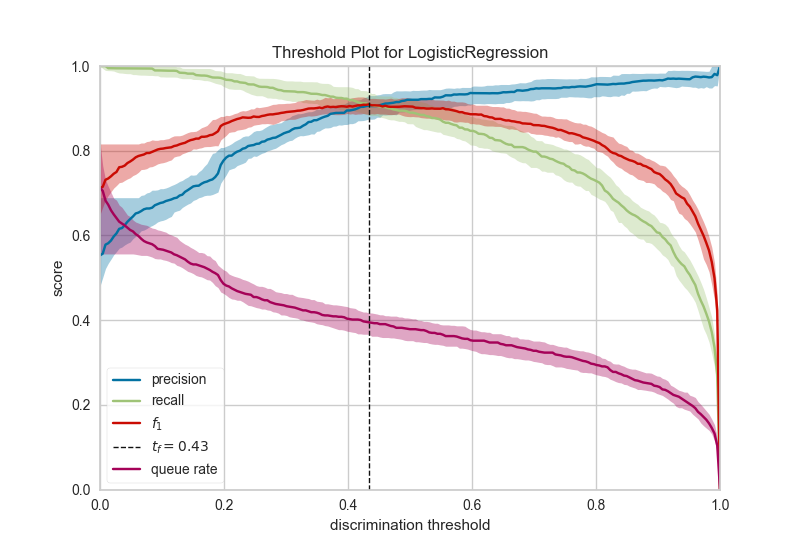
\includegraphics[scale=0.7]{resources/4/discriminationThresholdVisualization}\\
\subsection{Areas - or bands - around the curves}
The model will split the data multiple times, differently, into train and test sets and then run the trials. This ensures a certain amount of variability being visualized. Corresponding section on the site: \\

``\textit{The visualizer also accounts for variability in the model by running multiple trials with different train and test splits of the data. The variability is visualized using a band such that the curve is drawn as the median score of each trial and the band is from the 10th to 90th percentile.}''

\subsection{Queue rate}
``This metric describes the percentage of instances that must be reviewed.''\\
It can be helpful to think about the costs of reviewing whatever it is that must be reviewed in the context of business decision, where the ability to review is a limited resource and might be a factor in adjusting the threshold in order to find a favourable outcome.
\end{document}